
\documentclass[border=0pt]{standalone}
\usepackage{tikz}
\usetikzlibrary{shapes.geometric, positioning, calc}
\usetikzlibrary{decorations.pathreplacing}
\usepackage{amsmath}
\usepackage{pgfplots}
\pgfplotsset{compat=1.8}
\usepgflibrary{shadings}
\usepackage{xcolor}
\usetikzlibrary{arrows.meta, bending}
\usepackage{microtype}
\usepackage{lmodern}

\definecolor{navyblue}{HTML}{8babf1}
\definecolor{ol}{rgb}{1, 0.8, 0.5}
\definecolor{oh}{rgb}{1, 0.35, 0.5}

\begin{document}

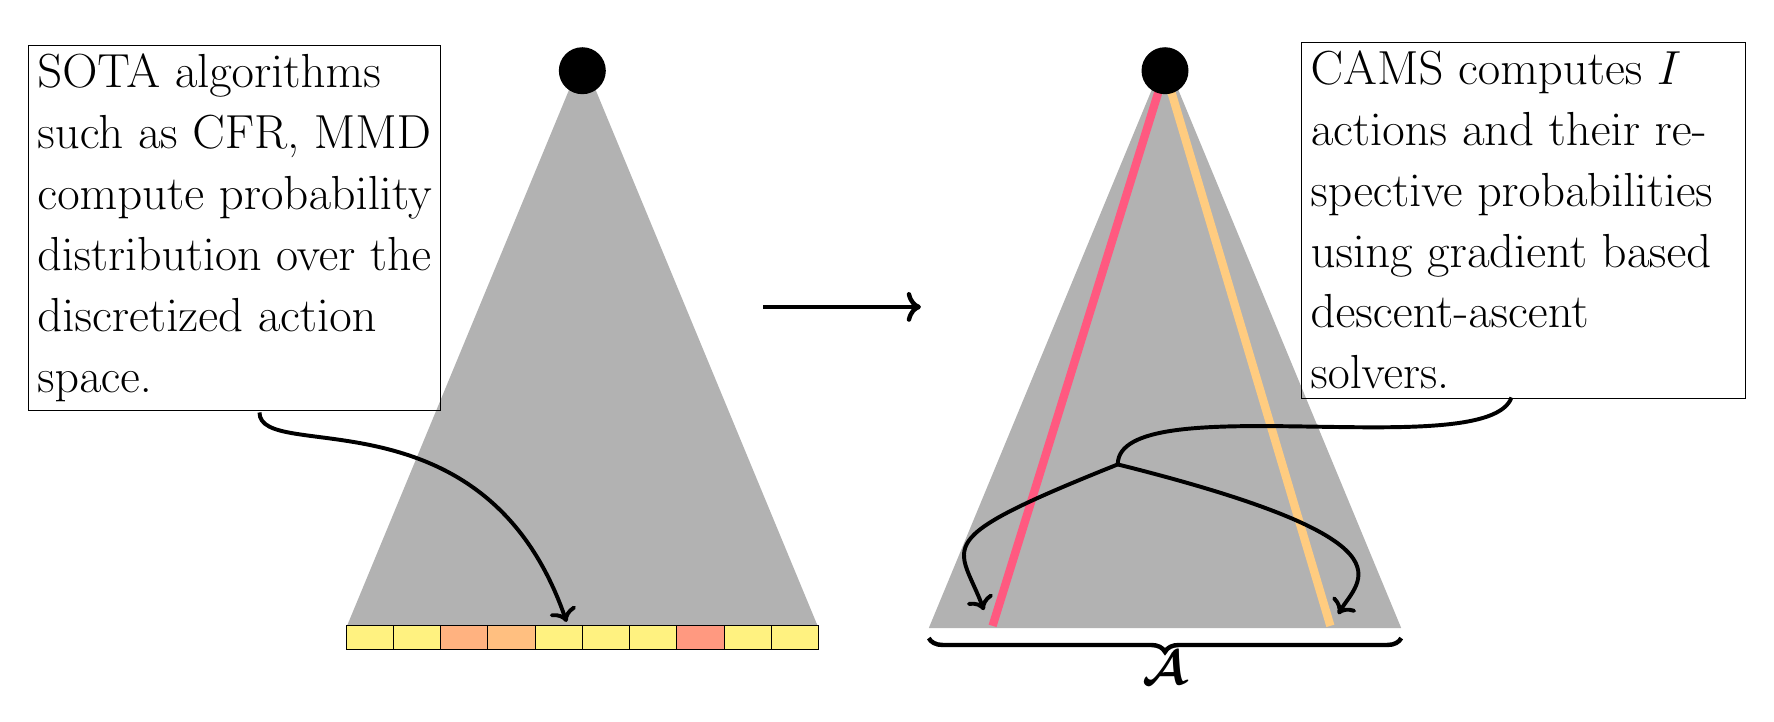
\begin{tikzpicture}[every node/.style={font=\normalsize}]
\tikzstyle{every node}=[font=\LARGE]
    % Original figure
    \begin{scope}[shift={(2.6, 0)}, scale=3]
        % Left tree (SOTA methods considering all actions)
        \node[isosceles triangle, rotate=90, fill=gray!60, minimum size=6cm, behind path] (B1) at (0.2, -1.7){};
        
        % Probability distribution with higher values for specific boxes
        \foreach \i/\prob in {0/0.05, 1/0.05, 2/0.3, 3/0.25, 4/0.05, 5/0.05, 6/0.05, 7/0.4, 8/0.05, 9/0.05} {
            \pgfmathsetmacro{\shade}{1 - \prob} % Invert probability for lightness
            \definecolor{cellcolor}{rgb}{1, \shade, 0.5} % Orange with varying shades
            \fill[cellcolor] ({-0.8 + \i*0.2}, -2.45) rectangle ({-0.8 + (\i+1)*0.2}, -2.35);
            \draw ({-0.8 + \i*0.2}, -2.45) rectangle ({-0.8 + (\i+1)*0.2}, -2.35); % Grid lines
        }
        \node[circle, fill=black, inner sep=6pt, label=above:{}] (A1) at(0.2, 0){};
    \end{scope}
    
    \node[draw,text width=5cm] at (-1.22,-2) (B1) {SOTA algorithms such as CFR, MMD compute probability distribution over the discretized action space.};

    \draw [black,line width=0.5mm,-{Computer Modern Rightarrow[flex'=.75]}]
        (-0.9, -4.34) .. controls (-0.9,-5) and (2, -4) .. (3, -7);
     % Right arrow
    \draw[->, ultra thick, ] (5.5, -3) -- (7.5, -3) node[midway, above] {};
    % Shifted copy of the figure
    \begin{scope}[shift={(10, 0)}, scale=3] % Shifted to the right by 3.5 units
        % Right tree (Shifted copy)
        \node[isosceles triangle, rotate=90, fill=gray!60, minimum size=6cm, behind path] (B2) at (0.2, -1.7){};

        \draw[-, color=oh, ultra thick, line width=3pt] (0.2, 0) -- (-0.53, -2.35);
        \draw[-, color=ol, ultra thick, line width=3pt] (0.2, 0) -- (0.9, -2.35);
        % % Probability distribution with higher values for specific boxes
        % \foreach \i/\prob in {0/0.05, 1/0.05, 2/0.3, 3/0.25, 4/0.05, 5/0.05, 6/0.05, 7/0.4, 8/0.05, 9/0.05} {
        %     \pgfmathsetmacro{\shade}{1 - \prob} % Invert probability for lightness
        %     \definecolor{cellcolor}{rgb}{1, \shade, 0.5} % Orange with varying shades
        %     \fill[cellcolor] ({-0.79 + \i*0.1985}, -2.45) rectangle ({-0.79 + (\i+1)*0.1985}, -2.35);
        %     \draw ({-0.79 + \i*0.1985}, -2.45) rectangle ({-0.79 + (\i+1)*0.1985}, -2.35); % Grid lines
        % }
        \node[circle, fill=black, inner sep=6pt, label=above:{}] (A1) at(0.2, 0){};
        
        \draw [ultra thick, decorate,decoration={brace,amplitude=5pt,mirror,raise=4ex}]
          (-0.8,-2.2) -- (1.2, -2.2) node[midway,yshift=-2.8em]{$\boldsymbol{\mathcal{A}}$};
    \end{scope}

    \node[draw,text width=5.4cm] at (15.15,-1.9) (B2) {CAMS computes $I$ actions and their respective probabilities\\using gradient based descent-ascent solvers.};
    
    % \draw [black,line width=0.5mm,-{Computer Modern Rightarrow[flex'=.75]}]
    %     (14.7, -3.9) .. controls (14.7,-5) and (12, -4) .. (12, -7);

    \draw [black, line width=0.5mm, -{Computer Modern Rightarrow[flex'=.75]}]
    (15, -4.15) .. controls (14.7, -5) and (10, -4) .. (10, -5) % Main arrow body
    .. controls (7.5, -6) and (8, -6) .. (8.3, -6.85); % Left branch

    \draw [black, line width=0.5mm, -{Computer Modern Rightarrow[flex'=.75]}]
    (10, -5) .. controls (14, -6) and (13, -6.5) .. (12.8, -6.9); % Right branch
\end{tikzpicture}

% \begin{tikzpicture}[level distance=1.5cm, sibling distance=2cm, 
%     every node/.style={font=\scriptsize}]

%     % Left tree (SOTA methods considering all actions)
%     \node[isosceles triangle, rotate=90, fill=navyblue!60, minimum size=2cm, behind path] (B1) at (0.2, -1.7){};
%     % \draw[top color=red] (-0.79,-2.45) rectangle ++(1.985, 0.1);

%     % Probability distribution with higher values for specific boxes
%     \foreach \i/\prob in {0/0.05, 1/0.05, 2/0.3, 3/0.25, 4/0.05, 5/0.05, 6/0.05, 7/0.4, 8/0.05, 9/0.05} {
%         \pgfmathsetmacro{\shade}{1 - \prob} % Invert probability for lightness
%         \definecolor{cellcolor}{rgb}{1, \shade, 0.5} % Orange with varying shades
%         \fill[cellcolor] ({-0.79 + \i*0.1985}, -2.45) rectangle ({-0.79 + (\i+1)*0.1985}, -2.35);
%         \draw ({-0.79 + \i*0.1985}, -2.45) rectangle ({-0.79 + (\i+1)*0.1985}, -2.35); % Grid lines
%     }
 
%     % \node[behind path, isosceles triangle, rotate=90, fill=gray!60, minimum size=0.8cm] (C1) at (-0.2, -1.6){};
    
%     % Label for action space |A|
%   %   \draw [ultra thick, decorate,decoration={brace,amplitude=5pt,mirror,raise=4ex}]
%   % (-0.6,-1.3) -- (0.2,-1.3) node[midway,yshift=-2.8em]{$\boldsymbol{|\mathcal{A}|}$};
  
%     % \node[below left= 0.1cm of C1] {$|\mathcal{A}|$};
%     \node[circle, fill=black, inner sep=2pt, label=above:{}] (A1) at(0.2, 0){};
%     % \node[circle, fill=black, inner sep=2pt, label=above:{}] (A2) at (-0.2, -0.95){};

    
%     \node[isosceles triangle, rotate=90, fill=gray!60, minimum size=0.8cm] (B1) at (2, -0.7){};
    
%     % add a right arrow
%     \draw[->, thick] (0.7, -1) -- (1.2, -1);
    
%     \node[isosceles triangle, rotate=90, fill=gray!60, minimum size=0.8cm] (B2) at (1.75, -1.6){};
%     \draw[-, blue, ultra thick] (2, 0) -- (1.75, -0.95);
%     \draw[-, blue, ultra thick] (2, 0) -- (2.3, -0.95);

%     \draw[-, blue, ultra thick] (1.75, -0.95) -- (1.6, -1.82);
%     % \draw[-, blue, ultra thick] (1.75, -1.2) -- (1.8, -2.4);
    
%     \node[circle, fill=black, inner sep=2pt] (O1) at (2, 0){};
%     \node[circle, fill=black, inner sep=2pt] (O2) at (1.75, -0.95){};
    

% \end{tikzpicture}

\end{document}